In order to demonstrate the construction of a neural network
potential, this chapter will demonstrate the use of Tensorflow 
to reconstruct the Lennard-Jones potential.
The Lennard-Jones potential is the simplest
realistic molecular dynamics potential, and since it is a function
of only radial distance, symmetry functions are not required.
We can thus use neural networks to perform a simple regression
on a function accepting one input and producing one output.
This serves to illustrate some of the intuitions and problems
one runs into when using more complex methods such as 
atom-centered descriptors and gives a nice introduction into
modern Tensorflow. We will be using the Tensorflow 2.0
beta version recently released, since it introduces a wide array
of changes which will likely prove influential to the long-term
direction of the Tensorflow project.

\subsection{Tensorflow implementation}
The code used to produce this implementation is
a modification of the Tensorflow 2.0 for experts guide
which is available online\footnote{\url{
https://www.tensorflow.org/beta/tutorials/quickstart/advanced}}.
We start with some necessary imports from the Numpy and Tensorflow
libraries. Tensorflow from 2.0 onwards is now primarily accessed through
its Keras interface, which is a general high-level API for
constructing and training neural networks.
We also use a utility function from the scikit-learn library
for splitting the dataset into train and test data, but this is
merely for convenience as it is very simple to implement from scratch.
Finally we use the matplotlib and Seaborn libraries for
producing the plots.

\begin{minted}{python}
import numpy as np
import matplotlib.pyplot as plt
import seaborn as sns
import tensorflow as tf
from tensorflow.keras import Model
from tensorflow.keras.layers import Dense
from sklearn.model_selection import train_test_split
sns.set()
\end{minted}

Our neural network is a simple feed-forward artificial neural network
which inherits from the tensorflow.keras base model.
It contains 2 layers with 50 and 10 neurons respectively
using the hyperbolic tangent as the activation function.
The neural network produces a single output which represents
the potential energy and is computed as a linear function
aka a dot product of the activations in the final hidden layer
and the weights in the output layer.
The gradient of the neural network with respect to the input
can be computed using the tensorflow.GradientTape object.
The GradientTape monitors the computation from the input to the output
and is then able to backpropagate the output in order to obtain
the gradient.

\begin{minted}[firstnumber=last]{python}
class MyModel(Model):
    def __init__(self):
        super(MyModel, self).__init__()
        self.d1 = Dense(50, activation="tanh")
        self.d2 = Dense(10, activation="tanh")
        self.d3 = Dense(1, activation="linear")

    def call(self, x):
        x = self.d1(x)
        x = self.d2(x)
        x = self.d3(x)

        return x

    def derivative(self, x):
        with tf.GradientTape() as t:
            t.watch(x)
            y = self.call(x)

        return t.gradient(y, x)
\end{minted}

The data is produced using the Lennard-Jones potential,
which is a simple function of radial distance. The inputs
need to be in the shape of matrices in order
to be fed through the neural network in batches.
We split the data into train and test using a test fraction of 0.2,
with the remainder used for training.

\begin{minted}[firstnumber=last]{python}
def lennard_jones_data():
    lj = lambda r: 4 * ((1.0 / r) ** (12) - (1.0 / r) ** 6)

    x = np.linspace(0.90, 3.0, 10000).reshape(-1, 1)
    y = lj(x)

    x_train, x_test, y_train, y_test = train_test_split(
        x, y, test_size=0.2
    )

    return (x_train, y_train), (x_test, y_test)
\end{minted}

The data which is in the form of numpy arrays can easily
be converted into tensors which can then be processed
by Tensorflow. In order to perform regression
we will use the mean squared error for evaluating
the loss. We will use the Adam optimizer, which is currently
the most popular optimizer for training neural networks,
and generally outperforms the other less popular optimizers.

\begin{minted}[firstnumber=last]{python}
(x_train, y_train), (x_test, y_test) = lennard_jones_data()

train_ds = tf.data.Dataset.from_tensor_slices(
        (x_train, y_train)
).shuffle(1000).batch(32)
test_ds = tf.data.Dataset.from_tensor_slices(
        (x_test, y_test)
).batch(32)

model = MyModel()
loss_object = tf.keras.losses.MeanSquaredError()
optimizer = tf.keras.optimizers.Adam()

train_loss = tf.keras.metrics.Mean(name="train_loss")
test_loss = tf.keras.metrics.Mean(name="test_loss")
\end{minted}

The train and test steps are wrapped as Tensorflow functions
so that they can be efficiently called and applied to tensors.
For every train step the loss is computed and then backpropagated
so that the optimizer can apply updates to the weights and biases.
We subsequently train the neural network for 100 epochs, computing
the train and test loss for every epoch.

\begin{minted}[firstnumber=last]{python}
@tf.function
def train_step(images, labels):
    with tf.GradientTape() as tape:
        predictions = model(images)
        loss = loss_object(labels, predictions)
    gradients = tape.gradient(loss, model.trainable_variables)
    optimizer.apply_gradients(zip(gradients, model.trainable_variables))

    train_loss(loss)

@tf.function
def test_step(images, labels):
    predictions = model(images)
    t_loss = loss_object(labels, predictions)

    test_loss(t_loss)

epochs = 100

for epoch in range(epochs):
    for images, labels in train_ds:
        train_step(images, labels)

    for test_images, test_labels in test_ds:
        test_step(test_images, test_labels)

    template = "Epoch {}, Loss: {}, Test Loss: {}"
    print(template.format(
            epoch + 1, train_loss.result(), test_loss.result()
        )
    )
\end{minted}

\subsection{Comparison and relative error}

\begin{figure}[H]
    \centering
    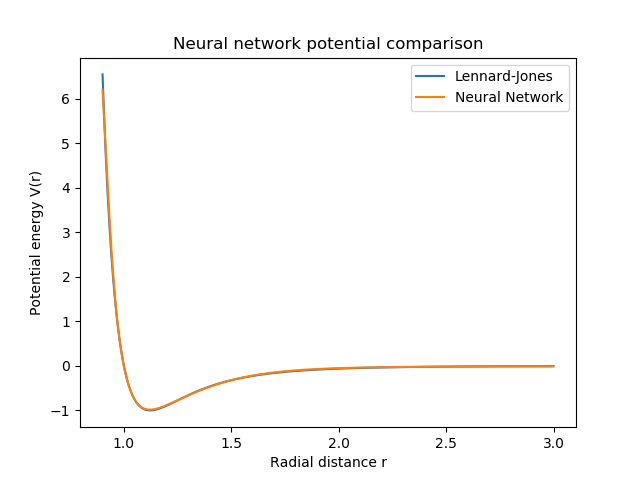
\includegraphics[width=\linewidth]{potential_comparison.png}
    \caption{Neural network potential compared to Lennard-Jones.}
    \label{fig:potential-comparison}
\end{figure}

\begin{figure}[H]
    \centering
    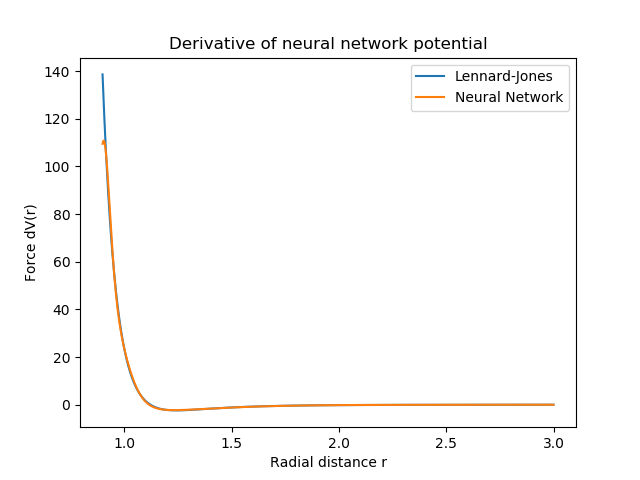
\includegraphics[width=\linewidth]{force_comparison.png}
    \caption{Neural network derivative compared to Lennard-Jones.}
    \label{fig:force-comparison}
\end{figure}

After training the network we can evaluate its performance
on test data. 
For the potential energy we obtain a root mean squared error of
$0.37$ (energy units).
However, the root mean squared error does not tell the complete story,
and the simplest way to evaluate the fit is to plot the potential.
In figure \ref{fig:potential-comparison} the neural network potential
is plotted with the Lennard-Jones potential.
We see that this potential is not difficult to reproduce,
as the number of datapoints is relatively small, and we used
a small number of epochs, amounting to only a few seconds of training.
The potentials agree very well on most of the input space, and we can
only spot a small divergence as the potential rises sharply
around a radial distance of one.

For the error in the derivative we obtain a force root mean squared error
of $61.7$ (energy units per length units), which is approximately two orders
of magnitude larger. The derivatives are plotted in figure
\ref{fig:force-comparison}.
The difference in derivatives is more pronounced, as the
difference is much larger as the radial distance decreases from
around one, and we can see that the neural network does not
have the same asymptotic behaviour. This poses a potential problem
for the dynamics, as the forces aka the derivatives keep
the atoms from moving too closely and causing massive
increases in the energy of the system.
This implies that we should train the potential on a representative
set of points in order to reproduce the correct asymptotic behaviour,
especially at the edges of configuration space.
It may also be beneficial to include force terms in the loss function,
as this is expected to decrease the error in the derivatives.

\begin{figure}[H]
    \centering
    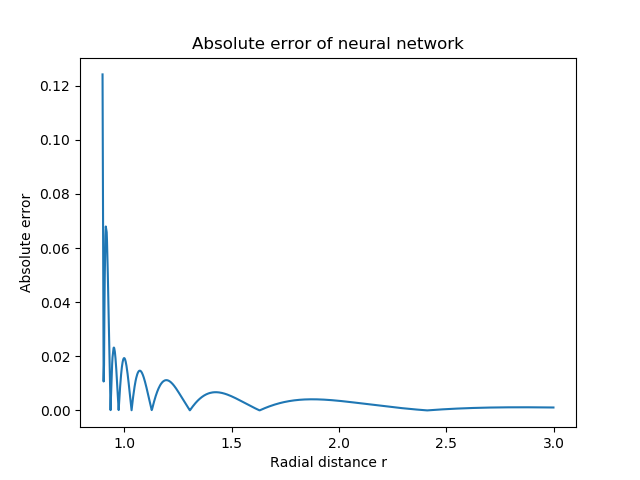
\includegraphics[width=\linewidth]{potential_absolute_error.png}
    \caption{Absolute error of the neural network potential compared
        to Lennard-Jones.}
    \label{fig:potential-rel-error}
\end{figure}

\begin{figure}[H]
    \centering
    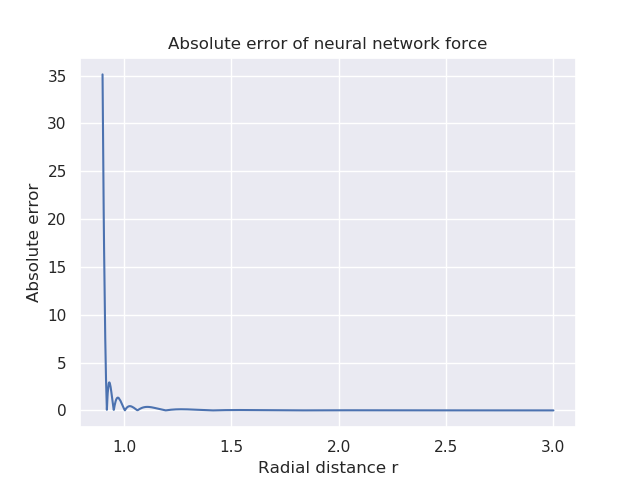
\includegraphics[width=\linewidth]{force_absolute_error.png}
    \caption{Absolute error of neural network derivative compared
        to Lennard-Jones.}
    \label{fig:force-rel-error}
\end{figure}

In figure \ref{fig:potential-rel-error} we have plotted
the absolute error of the neural network potential, defined
as $\left| E_p - E_{\text{NN}}\right|$
where $E_{\text{NN}}$ is the potential energy from the neural network.
From this we can see that the error in the fit is much larger
at one edge of configuration space, as shown in the above plots.
The neural network is able to reproduce small values
at larger distances, but not the asymptotic behaviour
as the interatomic distance approaches zero.
Additionally, we can observe that the absolute error in the derivative
is two orders of magnitude larger than the error in the potential energy fit.
However, since
this behaviour occurs only at the edge of the input space,
dynamics could be preserved by training on a representative set
of input data. This may also not be a big problem, as
with appropriate timesteps some configurations of interatomic distances
should never be observed in molecular dynamics simulations,
and would cause problems regardless of the accuracy of the
interatomic potential.
